
\documentclass[11pt,a4j]{jreport}

\usepackage{comment}
\usepackage{float}
\usepackage{color}
\usepackage{multicol}
\usepackage[dvipdfmx]{pict2e}
\usepackage{wrapfig}
\usepackage{graphicx}
\usepackage{bm}
\usepackage{url}
\usepackage{underscore}
\usepackage{colortbl}
\usepackage{tabularx}
\usepackage{fancyhdr}
\usepackage{ulem}
\usepackage{cite}
\usepackage{amsmath,amssymb,amsfonts}
\usepackage{algorithmic}
\usepackage{textcomp}
\usepackage{xcolor}
\usepackage[ipaex]{pxchfon}
\usepackage{booktabs}
\usepackage{multirow}
\usepackage{ulem}

\usepackage[top=30truemm,bottom=30truemm,left=25truemm,right=25truemm]{geometry}

\begin{document}

\thispagestyle{empty}
\begin{center}

\vspace{20mm}
{\Large\noindent 2024年度 卒業論文}\\
\vspace{40mm}
{\huge\noindent\textbf{警備員ロボットの抑止力向上のための}}\\
\medskip
{\huge\noindent\textbf{オペレータ支援システムの開発}}\\
\vspace{\baselineskip}
\vspace{40mm}

{\Large\noindent
2024年1月31日\\
\vspace{\baselineskip}
指導教員 神田  崇行\\
\vspace{\baselineskip}
京都大学工学部\\
神田研究室\\
\vspace{\baselineskip}
1029323422 天野岳洋\\
}
\vspace{40mm}

\end{center}

\thispagestyle{empty}
\clearpage

%=====================================================================================
\renewcommand{\abstractname}{要旨}

\begin{abstract}


アバターロボットが普及しアバターを介して遠隔地から勤務することが新たな働き方として認められつつある。通勤が必要ないため場所を問わず働けることが
大きなメリットであり、今後ますます普及することが予想される。
具体例では、スタッフ全員がアバターロボットのカフェ「分身ロボットカフェDAWN」\cite{takeuchi2020avatar}であったり、
ugo株式会社による警備アバターロボットugoの、ミツカングループや東北電力株式会社といった企業での導入例がある。
しかし、警備員のような人に指示する必要があるような仕事をアバターを介して行う際には大きな問題もある。
それは、アバターロボットに注意された際、人は実際の人間に注意されてるとは感じず、たかがロボットと侮ることが多く、直接注意する場合と比べて抑止力が低下するというものである。
そこで本研究では、認知的不協和理論に基づき、注意されたときに自分のもつ信条に関する認知と自分の行動に関する認知とが矛盾することによって生じる不快感と、
その解消方法に注目することによって、より効果的な注意文言を作成しそれらをオペレータに
提示することによって、オペレータの対応の質を高め、抑止力を向上させることを目的としたオペレータ支援システムの開発を行った。

具体的には、ロボットの移動操作の簡単化によって、
オペレータがより対話に集中できるようにすることに加えて、オペレータが相手が取ったであろう不快感の解消方法を判断し、
それに基づいて提示された注意文言の中で効果的なものを用いることで、よりアバターロボットの抑止力を強めることを可能にした。
この支援システムを用いることで、
操作に不慣れなオペレータであっても、より効果的にロボットを操作することができるようになるため、警備員の仕事を全うすることが容易になると考えられる。
\end{abstract}

%=====================================================================================

% 目次の表示
\tableofcontents


%=====================================================================================
\pagestyle{fancy}
\lhead{\rightmark}
\renewcommand{\chaptermark}[1]{\markboth{第\ \normalfont\thechapter\ 章~~#1}{}}
%=====================================================================================

\chapter{はじめに} %章

\section{研究背景} %1.1
本章では、現状アバターロボットが抱える問題について説明したのちに、その問題の解決のために用いた認知的不協和理論についての説明を行う。
\subsection{アバターロボットと抱える問題} %1.1.1
アバターロボットとは、人間が遠隔地に存在からロボットを操作することで、現地での作業をかのうロボットである。アバターロボットを遠隔地から操作することをテレオペレーションと呼ぶ。
アバターロボットは、リモートワークを可能にする。リモートワークについては、働く場所を問わないことから通勤の必要がないことや、時差を利用した業務が可能になることなどの長所があげられる。
加えて他の人間と直接接する機会が少ないことなどから、パンデミック時において、通常の働き方よりも有利である。またリモートワークは従業員だけでなく組織にとっても
利点があることがわかっている。例えば、\cite{FERREIRA202170}では、企業が地理的制約なしに優秀な人材を獲得できることや、
オフィスの維持費や交通費を削減できることがあげられている。さらに、
アバターロボットを使ったカスタマーサービスは、リモートで働けるだけでなく、
サービス業務をこなせることも報告されている\cite{Kanda2010}。他にも、身体障碍を持つ人が
アバターロボットを用いることによって、カスタマーサービスのような物理的な仕事を行うことができるようになる。
さらに、その際に、身体障碍を持つ人の社会参加感や精神的充足感をもたらすことがわかっている\cite{takeuchi2020avatar}。
そのため、アバターロボットを介した業務は教育、医療、サービス業等の分野で広く普及することが予想される。

それらの業務において、人々を注意し、特定の行動を抑止するという行為は重要である。例えば、教育の場面において先生は生徒に対して、集中力に欠ける行動をとっていた場合、注意することによって生徒の集中を取り戻すことができる。
またサービス業の場面においては、他の客に迷惑をかける行動を取る客がいた場合に、店員が注意することでその行動を防ぐことができる。
しかし、人を注意するという行為には注意が逆効果になったり、注意相手とのトラブルに陥ったりといったリスクも伴う。
ロボットを用いた場合、注意相手との直接のコミュニケーションが存在せずそれらリスクがないことから、ロボットは注意を行う際の便利なツールとなる。
以上のことから、種々の業務に存在する注意という行為にロボットは有用であると考えられるが、
単なる自律ロボットでは、人の柔軟なコミュニケーションに対応することは難しい。なぜならば、
人との円滑なコミュニケーションには、相手の表情や声のトーン仕草などを読み取り、相手の感情を推測することが必要であり、それらは現時点で自律ロボットには困難であるからである。
そこで、単なる自律ロボットではなくアバターロボットが用いられる。

しかし、ロボットによる注意にも人間によるそれとは異なった問題点もある。それは、不慣れな場合に操作が難しいことと抑止力の面において劣るという点である。
ここで抑止力とは、歩きスマホのような社会的規範に背くような行動をしている相手に対して、
注意した際にどれくらいの人がその行動をやめるかを意味するものとする。
操作に関してロボットの最大速度は安全のために通常の人の歩行速度より低めに設定されていることが多く、
そのために移動操作にストレスを感じる場合がある。抑止力に関して例えば\cite{Mizumaru2019}において、歩きスマホをしている人に対してロボットが注意を行った時に、
一般的な近づき方をした場合に11人中9人が無視し、工夫をした近づき方であっても13人中5人が無視し引き続き歩きスマホを続けていた。
これは人が直接注意した場合と比べて明らかに少ない。
本研究では、この課題に取り組む。ここで注意されたときの人が行動をやめる理由を次のように仮定した。
Festingerによる認知的不協和理論\cite{Festinger1957}に基づき、
注意されたことによって
自分の行動と自分の信条とが矛盾することに気付かされ、その矛盾によって不快感が生じ、その解消のために行動をやめる必要があるからであると仮定する。
以上の仮説のもと、認知的不協和理論における「行動をやめる」以外の解消方法に注目した。

\subsection{認知的不協和とは} %1.1.2
\label{sec: CDT}
認知的不協和理論\cite{Festinger1957}とはFestingerにより提唱された理論であり、人間が互いに相反する認知を抱いた場合、その状態(不協和)に不快感を感じ
その不快感の解消のために、不協和の解決を図るというものである。
この認知とは、行動、知覚、態度、信念、感情といった様々な事象に関するものであり、多くの場合片方の認知は自らの行動に関するものである。
例えば、表\ref{fig: CDTExample}のようにたばこは健康に良くないと分かっているのに、タバコを吸ってしまった際に生じる不快感が認知的不協和である。
この不快感は、認知1と認知2が矛盾しているために、生じるものである。
\begin{table}[H]
  \centering
  \begin{tabular}{c|c}
      認知1 & たばこは体に害をもたらす  \\ \hline
      認知2 & 私はたばこを吸っている \\ 
  \end{tabular}
  \caption{認知的不協和の例}
  \label{fig: CDTExample}
\end{table}


この不快感を解消するために、いくつかの選択肢をとることができる。
\begin{enumerate}
  \item 行動を変える
  \item 認知を変える
  \item 新たな認知の追加を行う
  \item 矛盾の矮小化、無視
\end{enumerate}
それぞれについて、たばこの例で具体的に説明を行う。
\subsubsection{行動を変える}
行動を変えることは、たばこを吸うのをやめることであり、表\ref{fig: CDTExample}の認知2の変化をもたらすことにより、表\ref{fig: ReduceDissonanceAction}のように変化し、認知1と認知2の不一致を解消することができる。
行動の変更が容易なものであれば、この方法をとることが最も理論的であるが、行動の変更が困難な場合もある。そのような場合、
この方法ではなく、他の方法をとることになる。
\begin{table}[h]
  \centering
  \begin{tabular}{c|c}

      認知1 & たばこは体に害をもたらす  \\ \hline
      認知2 & 私はたばこを\sout{吸っている}吸わない \\
  \end{tabular}
  \caption{行動を変える例}
  \label{fig: ReduceDissonanceAction}


\end{table}

\subsubsection{認知を変える}
認知を変えることは、表\ref{fig: CDTExample}の認知1を「たばこは体に害をもたらさない」とすることである。これにより、表\ref{fig: ReduceDissonanceChange}のように変化し、
実際に行動を改めることなく、認知1と認知2の不一致を解消することができる。
\begin{table}[h]
  \centering
  \begin{tabular}{c|c}
      認知1 & たばこは体に害を\sout{もたらす}もたらさない  \\ \hline
      認知2 & 私はたばこを吸っている \\
  \end{tabular}
  \caption{認知を変える例}
  \label{fig: ReduceDissonanceChange}
\end{table}
\subsubsection{新たな認知の追加}
新たな認知の追加を行うことは、表\ref{fig: CDTExample2}の認知3や認知4を追加することであり、
この追加によって、認知1と認知2の不一致度合いを軽減させることができるため、生じる不快感が小さいものとなる。
\begin{table}[h]
  \centering
  
  
  \begin{tabular}{c|c}

      認知1 & たばこは体に害をもたらす  \\ \hline
      認知2 & 私はたばこを吸っている \\ \hline
      認知3 & 喫煙をやめると他の人にあたってしまい迷惑となる \\ \hline
      認知4 & たばこを吸っていて長寿の人もいる \\ 
  \end{tabular}
  \caption{新たな認知の追加の例}
  \label{fig: CDTExample2}

\end{table}
\subsubsection{矮小化、無視}
矮小化、無視では認知自体を変えずに不協和を解消する方法である。このとき、注意してきた対象や
認知同士が生む不協和が矮小化もしくは無視されることになる。例えば、そもそも\ref{fig: CDTExample}の認知1と認知2が
それほど矛盾していないと思い込むことによって、生じる不快感を軽減することができる。
\vskip\baselineskip
ここで、本研究では上記方法が一つ取られた時点で、不快感が十分に解消されそれ以上の方法をとることがないことを仮定する。
よって不協和による不快感が生じた人は、上記の方法のうちいずれか一つをとることになる。

\section{研究目的}
本研究では、アバターロボットが抱える上記の問題を解決するために、有効な注意文言の提示と移動操作を簡単化する
オペレータ支援システムを開発する。その後、その支援システムを用いていくつかの実験を行い、
評価することを目標とする。本研究では以降、警備員の業務を想定し注意すべき行動を簡単のために、研究\cite{Schneider2022,Mizumaru2019}と同じように
歩きスマホのみとした。これは、歩きスマホが社会的規範に背くもっとも普遍的な行動であると考えられるためである。

有効な注意文言に関して、
人はある行動を注意されたときに生じる不快感をその行動をやめるのではなく、認知の変更や追加によっても解消できる。
その際に、注意された行動は引き続き行われることになる。
そこで、それらの解消方法に対抗する注意文言を用いることによって、人々の行動の変化を促すことができるはずである。
また移動操作に関して、注意を行うためには継続して対象の近くにいる必要があるが、それに集中するあまり対話がうまく行えないという問題があることが
予備実験からわかった。この予備実験では、歩きスマホをしている客に対して注意を行うことを目的に行った。
その際に、ロボットが人に追いつくためには人の将来いるであろう位置に移動する必要がある。そのため、ロボットはその対象現在位置ではなく
予測位置をむくことになり、結果その人を画角から外す必要があった。しかし、それでは今その人がどこにいるかわからないまま、
おそらく来るであろう位置に移動を続けなければならない。また、人と対話できる距離追いつけたとしても、
その人と対面するためにロボットの向きを変えなければならず、これらの操作は困難であり操作に集中する必要があった。
そこで、移動操作を支援するシステムの開発を行う必要が生まれた。


これら移動操作のサポートと、効果的な注意文言を提示するオペレータ支援システムを開発することによって、
不慣れな操作者であっても、より効率的に警備員の業務を行えるようになることを目指す。



\chapter{関連研究}
このセクションでは、HumanRobotInteraction(HRI)における認知的不協和理論を適用した研究を紹介する。その後に、歩きスマホを注意しやめさせるといった、人の行動に影響を
与えるために否定的なフィードバックや行動をとるロボットに関する研究について紹介を行う。そして開発するシステムのようなテレオペレーション支援に関する研究
について様々な例と本研究との差異について説明を行う。
\section{認知的不協和のHRIへの適用研究}
HRI分野において、認知的不協和理論の適用例を示す。例えば、研究\cite{washburn2022exploring}では、
人間が荷物配達ロボットに対して従順になる理由の説明として、認知的不協和理論を用いている。具体的には、
人間がロボットにタスクを依頼された場合に、人間が「タスクを果たすことを楽しいことだ」という認知を追加する傾向があることを
人間がロボットに対して従順になりやすいことの説明としている。また他にも、研究\cite{herse2018you}では、ロボットがわざと
最適ではない選択肢を人間に提供した際に、信頼されているロボットのほうがそうでないほうよりも、人間が反応を返すまでに
長い時間がかかることを示している。これの説明として、人間がロボットを信頼している場合に、ロボットが不適切な選択肢を提示した際に、
不協和が生じ、意思決定時に余分な負荷がかかるために、反応時間が長くなるという説明を行っている。しかし、これらのように多くの研究は、
あくまで結果の説明のために、認知的不協和理論を用いているものであり、ロボットがとるべき戦略を決定するために用いているものではない。

認知的不協和に基づく不快感を戦略として利用した歩きスマホの注意を行っている研究は存在している\cite{Schneider2022}。
しかし上記研究では自律ロボットを前提としており、認知的不協和の解消方法に関して、\ref{sec: CDT}章で述べた解消方法の内
どれを用いているかのその場での分別は難しいものとしており、行動をやめるか、ロボットの矮小化を行うことを仮定している。これは
アンケートに基づき、歩きスマホを行っている人が注意された際に用いる「行動を変える」以外の不快感の解消方法として、
ロボットの矮小化が多かったためである。例えば、
ロボットが機械音声を用いているために、ただのガイダンスだと捉えられたや、ロボットがただの機械であると捉えられたなどである。
そのため、一度単に「歩きスマホは危険なのでおやめください。」と注意されたが引き続き歩きスマホを行っている人に対して、
「あなたは私のことをただのロボットだと思っているかもしれませんが、私はみなさんのために働いているのです」と一律に話しかけることによって、ロボットの矮小化
を防ぐことを試みている。一方で本研究ではアバターロボットを用いるため、オペレータとして人間が操作することを前提としているため、
より柔軟な戦略を取ることが可能である。そこで、使用されたであろう解消方法に基づいて異なる文言を提示することで、より効果的な注意を行うことができるのではないかと考える。

\section{説得のために否定的なフィードバック・行動をとるロボット}
まずはじめに、説得は人の行動になにかしらの影響を与えるために行われるものであり、
本研究で取り組む抑止は特にその中でも、特定の行動をやめさせるための説得行為を指すものとする。
ロボットがいかにして人間に対して行動の変容をもたらせるかについては多くの先行研究で取り組まれている。一般的な研究課題は、
ロボットの行動やフィードバックがどのように人間の行動に変化をもたらすことができるかを明らかにすることである。
例えば、ロボットが人間とのじゃんけんゲーム内でわざと負けることによって贈賄を行い、その後人間がロボットにお願いされた
追加のタスクを行うかどうかについての研究\cite{sandoval2016can}では、ロボットがわざと負けた場合に(贈賄を行った場合)より好感度が高く、
しかし、追加のタスクについてはより非協力的になることがわかっている。また、他にも仮想的な洗濯作業中に省エネを促す際に、否定的なフィードバックをとるほうが、
肯定的なフィードバックよりもより効果的に人間に行動の変容をもたらすことがわかっている\cite{Midden2009}。ここで否定的なフィードバックでは、
エネルギーを使いすぎた際に批判や落胆を表現するものであり、肯定的なフィードバックでは、エネルギーを節約した際に褒めるといったものである。
また、研究\cite{paradeda2019makes}では、被験者が自律ロボットから助言を受けながら、決断を下すようなシチュエーションにおいて、ロボットが怒り等の負の感情を
表現すると、被験者はロボットのアドバイスに従う可能性が高くなり、説得が効果的になることが報告されている。しかし、
一般的にどのようなフィードバックが最も説得力があるかという研究課題に対する明確な答えはなく、それは実験のシチュエーションや人間と
ロボットの関係性によって異なる。多くの研究では、事前に定められた二つのフィードバック手法を比較してどちらがより
効果的かどうかについて調査しており、ロボットのフィードバックに対する人間の反応によって、その後のロボットの行動を
変化させる戦略をとるような研究は少ない。そこで、本研究では、相手のとった行動に対して次の発言内容を決定するような柔軟な戦略についての研究を行う。
\section{テレオペレーション支援に関する研究}
テレオペレーション支援に関する研究は多く行われており、様々な面から種々のシステムが開発されてきた。
例えば、\cite{chen2007human,triantafyllidis2020study}では、テレオペレーションにおいて課題となっている視野の狭さや方向感覚の喪失といった問題を、
視覚だけでなく聴覚や触覚などの他の感覚を利用する多モーダルインターフェースによって解決を試みている。
また、多数の無人航空機を操作する際にパフォーマンスを向上させる
ようなコントローラーへのハプティックフィードバック手法についての研究\cite{son2011measuring}などがある。
へパティックフィードバックとは、コントローラーの利用者に力や振動によって警告等を行うフィードバック手法のことである。
他にも、鉱業におけるテレオペレーションにおいての、
ユーザーインターフェースについての研究\cite{hainsworth2001teleoperation}や、
テレオペレーターが荒い言葉遣いで話したとしても意図認識を用いて、支援システムが丁寧な言葉遣いに変換するような支援システム\cite{Daneshmand2023}などいろいろなものが研究されている。
しかし、これらの研究のように大半では主に操作や発言の支援を行うものであり、それらの操作内容や発言内容は操作者が決定しなければならず、オペレーターは
どういった操作、どういった発言が効果的かを考える必要がある。
そこで、本研究では
警備員業務の中での注意時に有効な知識をオペレータに提示し、
オペレータはどのような文言が効果的かについて知らずとも、
自分で考える必要なく有効な注意喚起を行うことが可能になるような
支援システムの開発を目標とする。


\chapter{提案手法}



アバターロボットを用いて警備員の仕事を行うことを効率的に簡単に行うことを可能にするために、
注意文言の提示と画像\ref{pic:interface}のようなインターフェースを用いて捜査支援を行うシステムを開発した。
また注意文言については、先ほど述べたように歩きスマホに対する注意に関してのみを扱っている。
この章ではそれぞれについての詳細を述べる。

\section{不快感の解消方法に基づく注意文言の提示}
認知的不協和理論に基づいた注意文言の検討を行う。ここで目標となるのは、相手の歩きスマホという行動を
なるべくやめさせる文言を作成することである。
\subsection{生じる不快感}
\label{sec: dissonance}
\begin{figure}[htbp]
  
  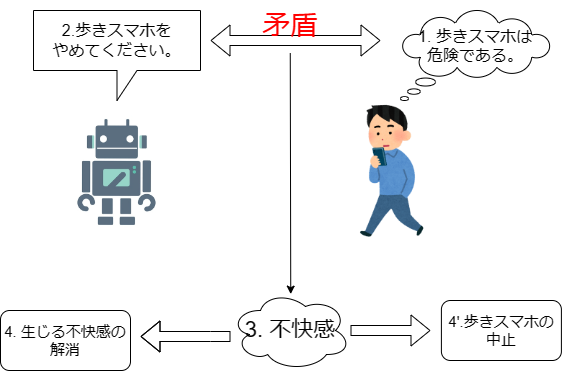
\includegraphics[width=13cm]{img/CDT.png}
  \caption{不快感が生じるまでの流れ}
  \label{fig: dissonance}
\end{figure}

多くの人が歩きスマホのことを危険だと考えており、さらに注意された際に不快感が生じることは示されている。
\cite{Schneider2022}では具体的に、人が歩きスマホを注意されたとき、図\ref{fig: dissonance}のように、以下のような過程を経ることが示されている。
\begin{itemize}
  \item[(1)] 歩きスマホをしている人も信念として、歩きスマホが危険であるという信念を持っている。
  \item[(2)] ロボットが注意を行う。
  \item[(3)] 自分の行動と信念とが矛盾していることに気付かされ不快感が生じる。
  \item[(4)] 歩きスマホをやめる。(4')歩きスマホをやめる以外の不快感の解消方法をとる。
  \label{item: dissonance}
\end{itemize}
ここで、(4)ではなく(4')の行動を行った相手に対して、その解消方法に応じた
追加の注意喚起によって、(4)の行動をとらせることを目指す。

\subsection{考えられる不快感の解消方法と有効な注意文言}
\label{sec: dissonance2}
前節\ref{sec: dissonance}で述べたように、歩きスマホをしているは注意された際に不快感が生じる。
\begin{table}[h]
  \centering
  
  
  \begin{tabular}{c|c}

      認知1 & 歩きスマホは危険である  \\ \hline
      認知2 & 私は歩きスマホをしている \\ 
  \end{tabular}
  \caption{歩きスマホによる不快感}
  \label{fig: UsingPhone}
\end{table}
この不快感は、図\ref{fig: UsingPhone}の、認知1と認知2が矛盾しているために生じるものである。
\ref{sec: CDT}章で述べたように、不快感を解消するために、いくつかの選択肢をとることができる。これらの選択肢の内、
1.行動を変えるという選択肢をとらせることが本システムの目標である。そのために、それ以外の選択肢をとった際に、その解消方法を無効にするような文言や、
新たに不快感を生じさせるような文言によって、再度不快感を解消する必要性を生み、1.行動を変えるという選択肢をとらせることが可能になると考える。

\subsubsection{行動を変える}
行動を変えることは、歩きスマホをやめることであり、この場合これ以上注意を行う必要はない。
\subsubsection{認知を変える}
認知を変えることは、表\ref{fig: UsingPhone}の認知1を「歩きスマホは危険ではない」とすることである。この認知の変更を困難にするためには、
再度歩きスマホが危険であるような認知を追加するような文言が有効であると考えられる。例えば、
「歩きスマホによる死亡事故例も存在します」や「歩きスマホによって他人をケガさせた場合、高額の賠償金を請求される可能性があります」
等があげられる。
\begin{table}[h]
  \centering
  
  
  \begin{tabular}{c|c}
      認知1' & 歩きスマホは危険\sout{である}ではない \\ \hline
      認知2 & 私は歩きスマホをしている \\ \hline
      認知3 & 歩きスマホによる死亡事故が存在する \\
  \end{tabular}
  \caption{認知の変更}
  \label{fig: AvoidDissonanceRevise}
\end{table}
そのような注意を受けた場合、表\ref{fig: AvoidDissonanceRevise}のように、認知3が追加される。
そして、認知1'と新たに追加された認知3の矛盾により新たに不快感が生じることとなる。
もしくは、認知1の変更が困難になる。それらの結果として、この方法での不快感の解消が難しく、再び不快感の解消を試みなければならない。
なので、この選択肢がとられた際に有効な
注意文言は、歩きスマホが危険であることを示す文言であると考えられる。
\subsubsection{新たな認知の追加}
不快感の解消のために、表\ref{fig: AvoidDissonance}の認知3や認知4が追加されることが考えられる。これらの認知は、
認知1と認知2の矛盾を軽減させることができるため、不快感の解消につながる。
\begin{table}[h]
  \centering
  \begin{tabular}{c|c}
      認知1 & 歩きスマホは危険である \\ \hline
      認知2 & 私は歩きスマホをしている \\ \hline
      認知3 & 地図アプリを見ており、これは必要な行為である \\\hline
      認知4 & 周りに人がおらず、他人に迷惑をかけていない \\ 
  \end{tabular}
  \caption{新たな認知の追加}
  \label{fig: AvoidDissonance}
\end{table}
そこで、これらの認知の追加に対しては、認知3の追加に対して「道案内なら私がしますよ。」や認知4の追加に対して
「そこの柱の裏から急に人が飛び出してくるかもしれません」といった文言が有効であると考えられる。
\begin{table}[h]
  \centering
  \begin{tabular}{c|c}
      認知1 & 歩きスマホは危険である \\ \hline
      認知2 & 私は歩きスマホをしている \\ \hline
      認知3 & 地図アプリを見ており、これは必要な行為である \\
      認知3' & 道案内を目の前の人に頼むことができる \\ \hline
      認知4 & 周りに人がおらず、他人に迷惑をかけていない \\ 
      認知4' & そこの柱の裏から急に人が飛び出してくるかもしれない \\ 
  \end{tabular}
  \caption{新たな認知の追加}
  \label{fig: AvoidDissonanceBlock}
\end{table}
なぜならば、これらの
文言は追加される認知と矛盾するものであり、図\ref{fig: AvoidDissonanceBlock}のように、認知3と認知3'の矛盾を生じさせることで、
新たな不快感が生まれる、もしくは、認知3の追加を防ぐことができると予想され、結果として、再び不快感の解消を試みなければならない。
よって、この選択肢がとられた際に有効な注意文言は、追加された認知に対して矛盾する文言であると考えられる。
そのためには、追加された認知を識別する必要があるが、これは人間のオペレータが存在することによって、
ある程度可能であることを前提としている。\footnote[1]{例えば、場所を探していそうならば、認知3の追加であるだろうし、周りに人がいないならば、認知4が追加される可能性が高い。}


\subsubsection{矮小化、無視}
ロボットが矮小化や無視の対象となることが多い\cite{Schneider2022}。そこで、この選択肢がとられた際には、
再度ロボットを無視することが困難になるような文言が有効であると考えられる。
そこで、対象の外見の特徴を述べたうえで注意することによって、ロボットの矮小化を防ぐことができると考えられる。
具体例として考えられる会話の例は、以下のような対話\ref{dialogue: Ignore}である。
\begin{table}[H]
  \centering
  
  
  \begin{tabular}{c|c}
      ロボット & 歩きスマホは危険ですので、おやめください。 \\ \hline
      人 & (無視) \\ \hline
      ロボット & そこの青いシャツを着ている方に言っています。 \\ 
  \end{tabular}
  \caption{矮小化・無視}
  \label{dialogue: Ignore}
\end{table}


\subsection{用意した文言}
以上のことから、システムが提示する注意文言は、表\ref{fig: Strategy}のようになった。
\begin{figure}[h]
  
  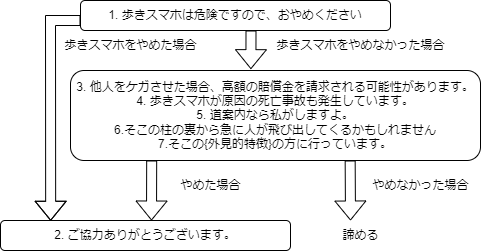
\includegraphics[width=15cm]{img/waystostop.drawio.png}
  \caption{注意文言}
  \label{fig: Strategy}

\end{figure}
まず、はじめに文言1を提示する。もし、人が歩きスマホをやめた場合には、文言2をいうように提示する。
また、歩きスマホを継続した場合には、それぞれとられた戦略によって、文言3,4,5,6,7のいずれかをいうように提示する。
その後歩きスマホをやめた場合には文言2をいうように、やめなかった場合これ以上の注意は行わない。
\section{移動操作の簡単化}
より人間らしい対話を可能にするために、発声はオペレータが行う。しかしながら、アバターロボットの移動操作に気をとられてしまい、
うまく対話が行えないという問題がある。そこで、移動操作を簡単にするためのシステム及びインターフェースを開発した。
システム全体の構成を図\ref{pic:systemcompose}に示す。これらのシステムを用いることによって、オペレータは画面クリックのような
簡単な操作で、アバターロボットを人の前まで移動させることと、可能な限りその人についていくことができる。このシステムによって、オペレータは歩きスマホをしている人の挙動に
集中できるようになり、さらにより人間らしい対話が可能になる。以下セクションでは、このシステムの構成について述べる。
システムではデータのやり取りはROSを介して行われる。ROSとは、ロボットのソフトウェア開発のためのライブラリであり、トピックのパブリッシュ、サブスクライブを用いて
データのやり取りを行うことができる。
%#TODO
\begin{figure}[H]
  
  \includegraphics[width=15cm]{img/system\_compose.drawio.png}
  \caption{移動支援システムの構成}
  \label{pic:systemcompose}

\end{figure}


\subsubsection{人位置計算}
既存のソフトウェアであるhuman\_trackerを利用しており、人物の位置を取得することができる。これは、ロボットに備わったLiDARセンサーから得られた点群データと事前に作成されたマップデータを用いており、
点群データの内から、マップデータに存在しないものを人としており、その人の位置を取得することができる。また、各人に対してidが割り振られ、このidは基本人に対して唯一である。
おおよそ1秒に5回から10回ほどの頻度で人位置と人idが発行され、このデータを用いて次の速度計算が行われる。

\subsubsection{速度計算}
各人idごとに、位置の時系列データから速度計算を行う。今回この速度計算は直近16個の位置データを用いて、前半8個の平均と後半8個の平均の差をとることで、速度を計算した。
これによって、各人の速度と、現在位置がわかる。そのデータを次のゴール計算に用いる。また、過去のデータ数が8個に満たない場合は速度計算を行わない。また、human\_trackerの仕様上、
異なる人であっても同じidが用いられることが時々起こりうるので、その場合は、過去に蓄えられた位置データをリセットしてから、追加を行う。この検出は、直近の位置データから大きく乖離している場合に、
異なる人であると判定を行った。

\subsubsection{ゴール計算}
ゴール計算では、ロボットの最大速度を事前定数として、ロボットの現在位置、各人の速度と位置を用いて、
各人と衝突することが可能かどうか、またその衝突位置を求めている。ここでの衝突は、会話できる距離にいることを意味しており、具体的には
人の進行方向120cm先にロボットがいる場合を衝突としている。具体的には以下の計算によって求められる。これは研究\cite{mumm2011human}において、
実験の中で人がロボットにもっとも近づいた時の距離が100cmから110cm程度であったことから、両者移動していることを考慮して、120cmとした。
人の位置を$H_x$, $H_y$とし、ロボットの位置を$R_x$, $R_y$とする。また、人の速度を$V_{hx}$, $V_{hy}$とし、ロボットの最大速度を$V_R$とする。また追いつくまでの時間を$t$とする。
これら用いた変数についてを表\ref{fig: variable}にまとめる。
\newcolumntype{C}{>{\centering\arraybackslash}p{3mm}}
\begin{table}[H]
  \centering
  \begin{tabular}{|c|c|c|c|}
    \hline
    人の位置 & 人の速度 & ロボットの位置 & ロボットの最大速度 \\ \hline
    $H_x$  $H_y$ & $V_{hx}$  $V_{hy}$ & $R_x$  $R_y$ & $V_R$ \\ \hline
  \end{tabular}
  \caption{変数について}
  \label{fig: variable}
\end{table}
この時、$t$秒後の人の位置は、$H_x + V_{hx}t$, $H_y + V_{hy}t$であり、この位置とロボットの初期位置との距離が$V_Rt$であるので、
以下の等式が成り立つ。\begin{equation}(H_x + V_{hx}t - R_x)^{2} + (H_y + V_{hy}t - R_y)^2 = V_R^2\end{equation}
これは$t$についての二次方程式なので、tについて解くことができる。この時、解の内正であるものが、衝突可能な時間となる。
二次方程式が実数の範囲で解けない、または、解が負の値となる場合は、衝突可能な時間は存在しない。また、衝突可能な時間が複数存在する場合は、より小さいほうを採用する。
この時間を用いて、衝突可能な位置を求めることができる。実際には、$H_x$, $H_y$の代わりに、数式\ref{eq: H'}の、$H'_x$, $H'_y$を用いて計算を行っている。
\begin{equation}
  \label{eq: H'}
\left\{\begin{array}{l}
H'_x = H_x + 1.2*\frac{V_{hx}}{\sqrt{{V_{hx}^2 + V_{hy}^2}}}\\
H'_y = H_y + 1.2 * \frac{V_{hy}}{\sqrt{V_{hx}^2 + V_{hy}^2}}
\end{array}\right.
\end{equation}
このようにすることによって、人の進行方向120cm先と衝突できるかどうか、またその際の位置を計算することができた。

\subsubsection{インターフェース}
ロボットに備え付けられたカメラから受け取った画像データをもとにして画像\ref{pic:interface}のようなインターフェースを作成した。
インターフェースでは、ゴール計算の際の各人に対して衝突可能かどうかを用いて、以下画像のように衝突可能な人は緑枠で、不可能な人は赤枠で囲むこととしている。このインターフェースを用いて、オペレータは
緑枠に囲まれた歩きスマホをしている人をクリックすることとなる。その際、ターゲットに選ばれた人を囲む枠は図のように太く塗られ、オペレータは今
だれを追跡しているかについて知ることができる。その後、クリックされた人のidをゴール計算に定期的に送る。そこで、ゴール計算では、そのターゲットidを受け取るたびに
送られていた人との衝突可能位置をゴールポーズとして発行する。ここでゴールポーズとは、目標となる位置と向きのことであり、その向きは
人の進行方向の180°回転した向きであり、ロボットと人が対面するようにしている。
\begin{figure}[H]
  
  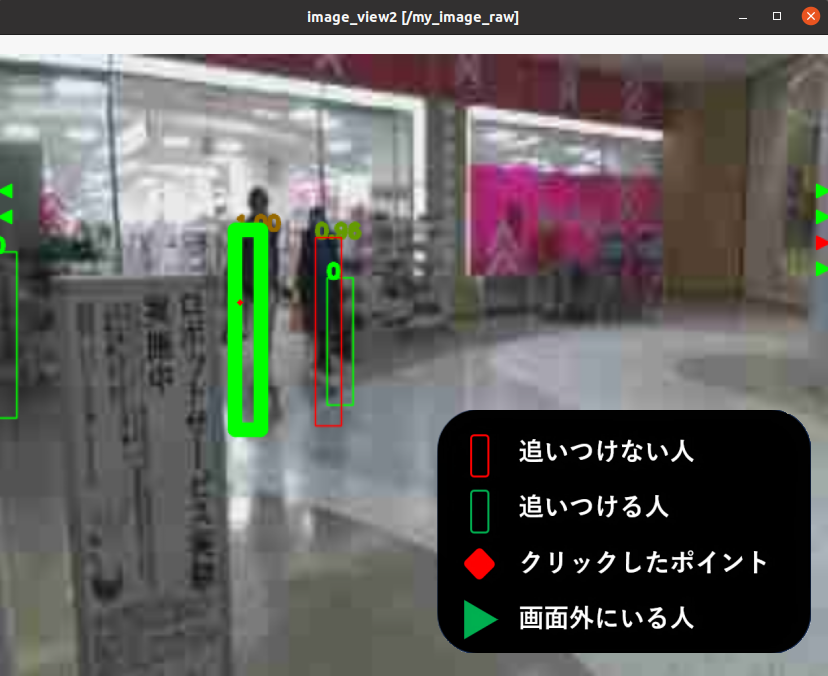
\includegraphics[width=15cm]{img/interface.png}
  \caption{操作支援インターフェース}
  \label{pic:interface}
\end{figure}
\subsubsection{移動方法計算}
既存のソフトウェアであり、発行されたゴールポーズを目指し障害物を避けながら、robotに対して移動速度、回転速度についての指令を行う。

%\subsubsection{メディア}
%media部分では、ロボットの備え付けられたカメラのデータ、マイクのデータを取得し、インターフェースに送る。また、オペレータの発した声
%を直接そのままロボットに備え付けられたスピーカーから出力する。


\chapter{評価実験}
\section{実験方法}
警備員の格好をしたアバターロボットを用い、大型のショッピングモール(ATC)の中で、歩きスマホをしている参加者に対して注意喚起を行った。また、注意喚起の際に、アバターロボットを操作するためのインターフェースを用いた。
実験の手順は以下のように行った。
\begin{enumerate}
  \item オペレータが用意したインターフェースを用いて、歩きスマホをしている人に近づく。
  \item 全ての人に対して、「歩きスマホは危険ですので、おやめください。」という注意喚起を行う。
  \item 歩きスマホをやめなかった場合、オペレータは反応から最も適切な注意文言を選択し再度注意喚起を行う。
  \item 歩きスマホをやめたか、またどの段階でやめたかについて記録する。
\end{enumerate}
TODO:画像挿入
\section{実験結果}
\section{考察}

\chapter{まとめ}
研究のまとめ。

%=====================================================================================
\chapter*{謝辞} %章を付けずにタイトル表示
\addcontentsline{toc}{chapter}{謝辞} %章立てせずに目次に追加するおまじない
本論文を作成するにあたり、みなさまに感謝の意を表します.

%=====================================================================================

\addcontentsline{toc}{chapter}{参考文献} %章立てせずに目次に追加するおまじない
\renewcommand{\bibname}{参考文献} %これがないと,タイトルが「関連図書」になってしまう
\bibliography{citation.bib} %bibtexファイルの読み込み
\bibliographystyle{jplain} %本文に\cite{}を入れることで,参考文献表示

\end{document}